\RequirePackage{luatex85}
\documentclass[12pt,letterpaper]{article}
\usepackage[utf8]{inputenc}
\usepackage{amsmath}
\usepackage[letterpaper,margin=1in]{geometry}
\setlength{\parskip}{5px}
\usepackage{url}
\usepackage{graphicx}
\graphicspath{{figures/}}
\usepackage{mathptmx}[ptm]
\usepackage[T1]{fontenc}
\usepackage{textcomp}
% \usepackage[scaled]{helvet}
\usepackage[compact,tiny]{titlesec}
\usepackage[backend=biber, style=nature, citestyle=authoryear, uniquename=init]{biblatex}
\usepackage{tikz}
\usepackage{wrapfig, framed}
\usepackage[font=small,labelfont=bf]{caption}
\usepackage[hidelinks]{hyperref}
\usepackage{listings}
\usepackage{relsize}
\usepackage[left]{lineno}
\usepackage{colortbl}

\pagenumbering{arabic}
\bibliography{alignpair_letter.bib}
\newcommand*\pct{\scalebox{.9}{\%}}
\newcommand{\red}[1]{\textcolor{red}{#1}}
\newcommand{\green}[1]{\textcolor{green}{#1}}
\newcommand{\blue}[1]{\textcolor{blue}{#1}}
\DeclareMathAlphabet{\mathcal}{OMS}{cmsy}{m}{n}
\hypersetup{
    colorlinks=true,
    linkcolor=black,
    urlcolor=blue,
    citecolor=black
}


% document begins here
\begin{document}
% \vspace*{0.35in}

% title goes here:
\begin{flushleft}
{\Large\textbf{COATi: }}
% codon-aware pairwise aligner + artifacts
\newline
% authors go here:
\\
Juan J. Garcia Mesa\textsuperscript{1,2},
Reed A. Cartwright\textsuperscript{1,3}
\\
\bigskip
1 Biodesign Institute, Arizona State University
\\
2 Ira A. Schools of Engineering, Arizona State University
\\
3 School of Life Sciences, Arizona State University
\\
\bigskip
* corresponding@author.mail

\end{flushleft}

% \abstract{Abstract}
\begin{abstract}
\noindent \textbf{Summary:} COATi is a statistical codon-aware pairwise aligner
that supports complex insertion-deletion models and is able to handle artifacts
present in genomic data.\\  % abstract summary can be longer.
\textbf{Availability:} The source code for COATi, along with documentation, is
freely available on GitHub: \url{https://github.com/CartwrightLab/coati} and is
implemented in C++.\\
\textbf{Supplementary information:} %\green{TODO}.
\end{abstract}


% now start line numbers
\linenumbers

\section{Introduction}

% sequence alignment is important and heavily used
Sequence alignment is a cornerstone step in bioinformatics
\parencite{sequence_alignment_rosenberg_2009}.
% errors in genomic data that lead to erroneous downstream analyses
Uncorrected errors in sequence alignment can lead to erroneous results in
functional and comparative genomic studies \parencite{estimates_schneider_2009}.
% to correct this common practice is to discard lots of data
Given that errors and artifacts are common in molecular data, this requires
costly curation practices that discard large amounts of information.
% despite available aligners, there is room for improvement
% summarize sentence into ~ "alignment is performed in the amino acid space"
In addition, a common strategy is to perform alignment inference in the amino
acid space \parencite{bininda2005transalign,abascal2010translatorx}.
While this approach is an improvement over DNA models, it discards information,
underperforms compared to alignment at the codon level, and fails in the
presence of artifacts such as frameshifts and early stop codons.
Although some aligners incorporate codon substitution models, they do not
support frameshifts or lack as statistical model.

% to address this, we present COATi
To address this problem, we present COATi, short for COdon-Aware Alignment
Transducer, a statistical pairwise aligner that incorporates codon substitution
models and is robust to artifacts present in genomic data.


\section{Description}

% Summarize pair-HMMs. Brief, comment typically used but move onto FST right away
Statistical alignment is typically performed using pairwise hidden Markov
models (pair-HMMs).
% This computational machines consist of two output tapes and a set of states that
% emit symbols onto one or both tapes.
Pair-HMMs have the ability to rigorously model molecular sequence evolution and
can calculate the probability that two sequences are related, represented
$P(X, Y)$ \parencite{yoon_2009_hmm}.
However, a limitation of pair-HMMs is the ability to only model evolution of two
related sequences from an unknown ancestor.
Finite-state transducers (FSTs) have the ability to calculate the probability
that a sequence $Y$ evolved from sequence $X$, represented $P(Y | X)$.
FSTs share similar computational benefits as pair-HMMs in addition to well
established algorithms for combining them in different ways
\parencite{bradley2007transducers}.
A powerful and versatile algorithm is composition, which consists of sending the
output one FST as the input of a second FST.
The FST model implemented in COATi is designed by composing smaller FSTs, each
representing a specific process.

% Evolution FST
Pairwise alignment in COATi is implemented via the Evolution FST (Fig.
\ref{fig:evolution-fst}), based on existing transducers (e.g.
\cite{holmes2001evolutionary}).
The Evolution FST is formed by composing a substitution FST that encodes a 64x64
codon model (Fig. \ref{fig:evolution-fst}-a) and an indel FST that models
insertions and deletions, including frameshifts (Fig. \ref{fig:evolution-fst}-b).
The innovation of the Evolution FST with respect to other transducers is the
combination of a codon substitution model that allows stop codons with gaps that
can occur at any position of any length.

\begin{figure}[h!]
\begin{framed}
\centering
    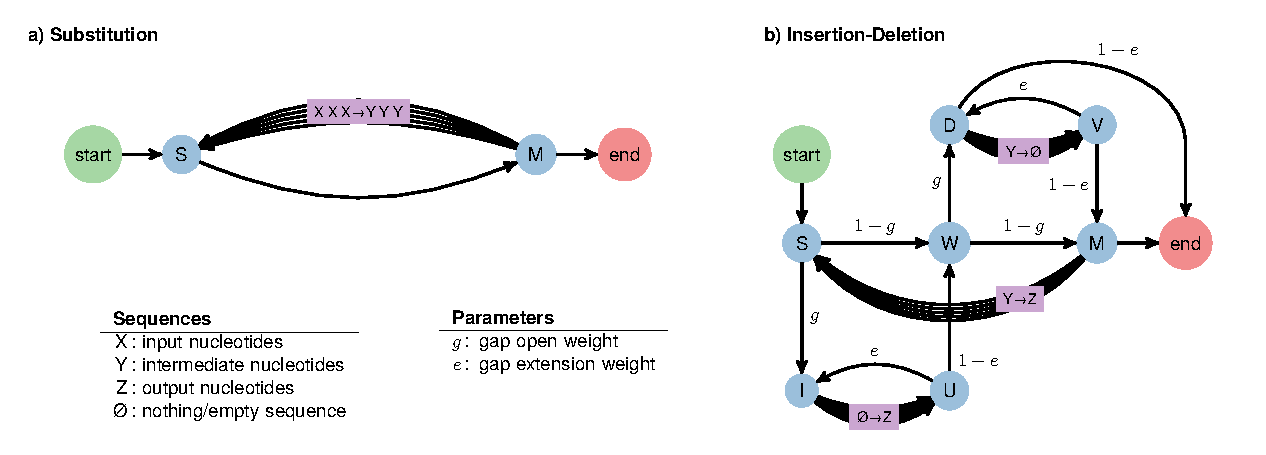
\includegraphics[width=\textwidth]{fig-evolution-fst.pdf}
    \caption{The Evolution FST is assembled by composing a substitution FST and
    an indel FST. Each node represents a state in an FST while arcs display
    possible transitions between states (and their weights). Absorption and
    emission of symbols occurs between states. (a) The substitution FST
    encodes a 64x64 codon substitution model with 64 arcs from M to S. (b)
    The indel FST allows for insertions (I to U) and deletions (D to V).
    Contiguous insertions and deletions are always arranged for insertions to
    precede deletions to limit equivalent alignments.}
    \label{fig:evolution-fst}
\end{framed}
\end{figure}


% FST implementation
% A path through the FST that \green{results} from composing both sequences with
% the Evolution FST represent a pairwise alignment.
% To find the most \green{probable/likely} alignment we must find the shortest
% path through.
The alignment FST is the result from composing both sequences with the Evolution
FST.
Any path through the alignment FST represents a pairwise alignment, while the
shortest path corresponds to the best alignment.
All FST operations including creation of models, composition, search for the
shortest path, and other optimization algorithms are performed using the C++
openFST library \parencite{allauzen2007openfst}.

% However, composing large FSTs is an expensive operation and can be prohibitive.
% Despite the existence of efficient C++ FST libraries (e.g. openFST
% \cite{allauzen2007openfst}), runtime is still limiting for sequence pairs longer
% than a few thousand nucleotides each.
% To solve this issue, the search for an optimal path (alignment) is
% reformulated as a dynamic programming problem.

% Evolution FST + Q matrix
% Marginal model? - Probably not
% DP - probably not
% 1 figure: FST model? - results table?


\section{Results}
% prelim data comparison?

Using 4000 human genes and their gorilla homologous pairs from the ENSEMBL
database \parencite{ensembl_hubbard_2002} we simulated a data set of pairwise
alignments with empirical gap patterns.
We used the data set to evaluate the accuracy of popular cutting edge aligners
Clustal$\Omega$ v1.2.4, %\parencite{clustal_omega_sievers_2011},
MACSE v2.06 \parencite{ranwez_macse_2011}, MAFFT v7.407, and
%\parencite{mafft_katoh_2002}
PRANK v.170427 % \parencite{prank_loytynoja_2014}
together with COATi.

After downloading, 1660 alignments contained gaps identified by at least one
aligner.
We randomly introduced gap patterns extracted from all five methods into the
2340 initially ungapped sequence pairs to generate the true alignments.
Alignment accuracy was measured using the distance metric $d_{seq}$
\parencite{metrics_blackburne_whelan_2011} between simulated and inferred
alignments.
In addition, accuracy of positive and negative selection was calculated
using the $F_1$ score by estimating $k_s$ and $k_a$ statistics.
% by estimating $k_s$ and $k_a$ statistics.

% % Software comparison table
% \begin{table}[!ht]
% \centering
%     %\frame{
%     % \begin{table}[h!]
% \begin{adjustbox}{width=\columnwidth,center}
\definecolor{bestcolor}{RGB}{230,230,230}

\begingroup\centering
\begin{tabular}{r|ccccc}
      & \textbf{COATi} & \textbf{MAFFT} & \textbf{PRANK\footnotesize{*}} & \textbf{MACSE} & \textbf{Clustal$\Omega$}\\
\hline
Method    & Trip-MG & DNA & Codon & DNA+AA & AA\\[2pt]
%\hline
Avg alignment error ($d_{seq}$) & \cellcolor{bestcolor}0.00214 & 0.01392 & 0.02001 & 0.01351 & 0.02691\\
Perfect alignments & \cellcolor{bestcolor}5722 & 5408 & 4706 & 2860 & 2937\\
Best alignments & \cellcolor{bestcolor}5152 & 4833 & 4748 & 3754 & 2595\\
Imperfect alignments & \cellcolor{bestcolor}1066 & 1380 & 2082 & 3928 & 3851\\
% \hline
F1 score of positive selection & \cellcolor{bestcolor}98.2\pct & 86.1\pct & 88.4\pct & 81.2\pct & 71.0\pct \\
F1 score of negative selection & \cellcolor{bestcolor}99.8\pct & 98.6\pct & 98.8\pct & 98.3\pct & 97.0\pct
\end{tabular}
\par\endgroup
% \end{adjustbox}
% \end{table}

%}
% 	\caption{Accuracy of COATi, PRANK, MAFFT, Clustal$\Omega$, and MACSE,
%             on 2340 simulated sequence pairs. Perfect alignments have
%             ($d_{seq}=0$), best alignments have lowest $d_{seq}$, and imperfect
%             alignments have $d_{seq}>0$ when at least one aligner found a
%             perfect alignment. Best values are highlighted in blue.}
% 	\label{table:comp}
% \end{table}

COATi was significantly (p < $1.714$x$10^{-8}$) more accurate at inferring
simulated alignments compared to other aligners according to the one-tailed
Wilcoxon signed ranked test, with an average alignment error ($d_{seq}$) value
of $6$x$10^{-4}$.
In addition, COATi produced more perfect alignments ($d_{seq}=0$), less imperfect
alignments, and more accurately retrieved events of positive selection (97.3\%).
Compared to COATi, MACSE (allows frameshifts) and MAFFT (using DNA) had an
average alignment error an order of magnitude larger than COATi ($6$x$10^{-3}$)
and a lower accuracy retrieving events of positive selection at a rate of 81.5\%
and 85.8\% respectively.
PRANK (using codons) and Clustal$\Omega$ (using amino acid translations) had
an average alignment error two orders of magnitude larger than COATi ($0.01$)
and a 87.3\% and 69.1\% accuracy retrieving events of positive selection,
respectively.
The accuracy retrieving events of negative selection was similar across all five
aligners (98.6\% $\pm$ 1.25\%).

% (Table \ref{table:comp}).



\section{Conclusions/Discussion}

COATi is an FST-based application that can find the optimal alignment between a
pair of sequences in the presence of artifacts using a statistical model.
% \green{(continue)}

\section*{Acknowledgments}

% The authors would like to thank \green{person1}, \green{person2}, and
% \green{number} reviewers for their helpful suggestions.

\subsection*{Funding}
This research was founded by an NSF-IIBR grant (\green{grant number}).\\

\noindent \textit{Conflict of interest:} none declared.

% \section{References}
% \printbibliography

\nolinenumbers

\end{document}
